\documentclass{tahquitz}

\begin{document}

\tableofcontents

\vfill\pagebreak

\discussionparindent

%=====================================================================

\section{Key to Symbols}

\vspace{10mm}


\includegraphics[width=\linewidth]{figs/key}

\vfill

\pagebreak

%=====================================================================

\section{Map of Fern Valley, Tahquitz and Suicide Rocks}

\vspace{10mm}

\includegraphics[width=\linewidth]{figs/large_area_map}

\vfill

\pagebreak

%=====================================================================

\section{Weather and Climbing Season}

Climbing season is usually from the end of March to mid- or late November. Often in early
spring there will be snow piled up at the bases of climbs, but the rock itself will be snow-free.
A webcam is available at \url{climbidy.com}.
For most of the summer, the forecast is for a 20\% chance of showers. Waiting for
the number to go to 0\% could mean not climbing all summer.

If checking the weather forecast for Idyllwild, keep in mind that the town is at 5400',
while the summit of Tahquitz Rock is at 7973'. As a rule of thumb, temperatures on north-facing
routes will feel colder by 20 degree F than the forecast in Idyllwild.
A forecast for the same elevation and area, including wind chill, is
available at \url{www.mountain-forecast.com/peaks/Jean-Peak/forecasts/2500}.

\section{Ratings}

\subsection{Historical}

The Yosemite Decimal System originated at Tahquitz, and the following
climbs were used as the standards to define the scale. For each climb, I've also listed the
consensus rating from Mountainproject (in 2015), which shows that there has been
quite a bit of inflation in the ratings over the years, mainly at the low end of the
scale --- nobody wants to say they climb 5.0 these days.

\begin{mytable}{Historical definition of the YDS, and inflation of ratings}
\begin{tabular}{llll}
5.0 & The Trough                        & FA 1936 & modern  5.4 \\
5.1 & Fingertip Traverse                & FA 1936 & modern  5.4 \\
5.2 & Frightful Variation of the Trough & FA 1944 & modern  5.2 \\
5.3 & East Lark                         & FA 1950 & modern  5.5 \\
5.4 & Angel's Fright                    & FA 1936 & modern  5.6 \\
5.5 & Ski Tracks                        & FA 1947, 1957 & modern  5.6, 5.9 \\
5.6 & Sahara Terror                     & FA 1942 & modern  5.7 \\
5.7 & Fingertrip                        & FA 1946 & modern  5.7 \\
5.8 & Mechanic's Route                  & FA 1937 & modern  5.8R \\
5.9 & Open Book                         & FFA 1952 & modern  5.9
\end{tabular}
\end{mytable}

\subsection{Evaluating ratings from a guidebook}

When depending on a guidebook for information about the difficulty of a climb, take
into account both the popularity of the climb and the date of its first ascent.
Old and lesser-known climbs often retain their historical ratings, which can be
extremely sandbagged by modern standards.

For example,
Summit magazine did a big spread on Tahquitz in 1960, which you can find scans of online.
They describe Northeast Farce as 5.3 and White Maiden's Walkway as 5.1. Having done
these two climbs, I would agree that Northeast Farce is a couple of grades harder
than the Maiden. But the 2001 edition
of the Vogel-Gaines guidebook rates these climbs as 5.3 and 5.4, respectively --- as if
the Maiden were the \emph{harder} climb. What has
probably happened is that because the Maiden is one of the most popular climbs on
the rock, there has been pressure to inflate its rating. Since almost nobody does Northeast
Farce, it retains the rating that was assigned when it was first climbed in 1954.

Another good example of this phenomenon is two obscure climbs on the inaccessible
south face of Suicide Rock, named Minor and Spring Cleaning. The first ascent of Minor is
lost in the mists of time, while Spring Cleaning had its FA in 1970. Several people who
I've done these climbs with agree that they are equal in difficulty, but Vogel and Gaines
list them as 5.1 and 5.6.

\pagebreak

\section{Descent routes}

\subsection{Friction descent}\label{subsec:friction-descent}

This is the class 3 standard descent for routes that end on the low western shoulder of the rock.
Most of these routes end below the friction descent, but some, such as White Maiden's Walkaway,
end above it.

Locate the house-sized boulder near the top of Tahquitz Rock's western shoulder,
perched above the south side of the rock. Pass around the boulder on either the
uphill or the downhill side. Insert into a chimney
leading down the south face of the rock, and then continue down a
chute/chimney that leads diagonally down and west.  Head east toward a
brushy island with a double pine tree. Continue traversing across
slabs until you reach the dirt.

Return to Lunch Rock on a use trail. This trail can become indistinct in spots,
and it is easy to be tempted into false alternatives that lead into dense
brush. The correct trail runs parallel to and just a few feet left of the
edge of the exposed granite. In most places the edge of the granite means the base
of the rock wall, but in two spots it means the edge of some low-angle
slabs. Stay off of these slabs, one set of which lies
below the friction descent
and another near the bottom of the Ski Tracks.

After passing the second set of slabs,
continue around the corner and back to Lunch Rock.

\subsection{North gully descent}\label{subsec:north-gully-descent}

This descent route is used by climbs that end near the top of the rock
or to its east. If coming down from the summit, scramble down class 3
rock to the saddle lying between the summit of Tahquitz Rock and
Tahquitz Peak. However, most of the climbing routes that use this descent end below and to
the east of the summit, and for these routes the traverse to the saddle is no more than
class 2.

Having reached the saddle, turn left down a steep, rough trail, then continue down slabs on the right.
Class 2. Get back on the use trail, which gradually becomes more obvious and well maintained.
Continue to the upper parking lot at Humber Park.


%%%%%%%%%%%%%%%%%%%%%%%%%%%%%%%%%%%%%%%%%%%%%%%%%%%%%%%%%%%%%%%%%%%%%%%%%%%%%%%%%%%%%%%%%%%%%%%%%%%%%%
% climbs
%%%%%%%%%%%%%%%%%%%%%%%%%%%%%%%%%%%%%%%%%%%%%%%%%%%%%%%%%%%%%%%%%%%%%%%%%%%%%%%%%%%%%%%%%%%%%%%%%%%%%%

\normalparindent

%------------------


\climb[1]{Angel's Fright}{5.6} %%%%%%%%% [1] is because this is the first one in the book

\topo{0.45}{angels_fright}

This short and popular climb was the original definition of 5.4 on the Yosemite Decimal Scale.
Most of the climb follows a long, uniform left-facing dihedral.
The start is almost directly above Lunch Rock. Pro to 2". FA
1936, Jim Smith and William Rice.

\pitch{1} This short pitch goes up an off-width chimney that is a little too
narrow to insert your whole body in but a little too wide for a thigh jam.
Two chock-stones provide convenient stances and natural pro, as well as helping
to confirm that this is the chimney you were looking for. 5.5

\pitch{2} This short crux pitch consists of steep face climbing with
possibly bewildering routefinding. Start up a ragged crack, then
exit right with a balancey move to a small ledge with a fixed pin.
Move back left and continue to a second piton, which is in bad condition
and starting to split in half. Climb to the right up a ramp to a big belay
ledge with two trees. The left-hand tree is festooned with slings. 5.6

\pitch{3} Cruise up the big dihedral that forms the backbone of the climb.
Most of the climbing is easy 5th class, but at the end a steep 5.5 headwall
stands between you and lunch ledge. Here the climb joins up with Fingertip Traverse
and Fingertrip. 55 m

%%% Pitches 4-5 are duplicated as pitches 5-6 of Fingertip Traverse and also in Fingertrip.

\pitch{4} Climb up from the middle of the ledge, surmounting all the steps
before traversing right. (Linking P4 and P5 will
give unacceptable rope drag unless you plan carefully.) 4th class.

\variation{1} For a more direct but harder route, step around a corner
to the right and then continue up.

\pitch{5} Move up and left on a flake
and then tiptoe along it as it continues around a corner.
This is easily protected with 0.3"-0.5" cams. (Do not follow the ramp lower down.) At a small
tree, head up a 5.4 slab with an orange bolt.

\variation{1} Head right into a 5.1 gully, then turn left at an overhang.

\variation{2} Climb a very thin finger crack, punctuated with pin scars. 5.6

Walk uphill to the friction descent route  (p.~\pageref{subsec:friction-descent}).
%=====================================================================

\climb{Fingertip Traverse}{5.4}

\topo{0.45}{fingertip_traverse}

An easy Tahquitz classic, this was the original climb used to define
5.1 on the Yosemite Decimal Scale. Most of the
climbing is 4th or easy 5th class, but the namesake traverse is more
like 5.4 by modern standards. Hike up to Lunch Rock and then head to the right along the
trail. The first pitch starts directly from the trail, near a 
truncated tree, with the first belay easily visible. Pro to 2". FA
1936, Jim Smith, Bob Brinton, Arthur Johnson, and William Rice.

\pitch{1} Scramble up to a large double oak tree in an alcove, the infamous
``ant tree.'' Anchor at the lower part of the tree to avoid stirring up
the ants. 30 m, 4th class.

\pitch{2} Move up the left side of the alcove's left wall, where it is
shortest, stemming against the opposite wall and then against two  branches
of the upper tree. Avoid the main trunk to keep from stirring up the ants.
Protect with a 0.3" cam (blue C4) in a small
finger crack before moving onto the rock. (This can also be done by
climbing higher up the tree, or by climbing the broken overhang at
the back of the alcove. These options can be protected with a 2" cam
in the crack in the left corner.) Continue up easy terrain. 30 m, 4th and easy 5th class
except for the committing move out of the tree.

\pitch{3} Climb a right-facing dihedral with good protection and
stances. Near the top of the dihedral, a short section requires laybacking (5.3).
Belay at a tiny ledge on a slab (small gear). 30 m

\pitch{4} Go around a corner and traverse along a finger-width crack,
smearing on the sloping face below, 5.4. Protect using the trees and
gear 1-2" and smaller. Continue up 4th-class terrain to Lunch Ledge (gear
belay). Here the route joins up with Angel's Fright and Fingertrip. 40 m

%%% Pitches 4-5 are duplicated as pitches 5-6 of Fingertip Traverse.

\pitch{5} Climb up from the middle of the ledge, surmounting all the steps
before traversing right. (Linking P5 and P6 will
give unacceptable rope drag unless you plan carefully.) 4th class.

\variation{1} For a more direct but harder route, step around a corner
to the right and then continue up.

\pitch{6} Move up and left on a flake
and then tiptoe along it as it continues around a corner.
This is easily protected with 0.3"-0.5" cams. (Do not follow the ramp lower down.) At a small
tree, head up a 5.4 slab with an orange bolt.

\variation{1} Head right into a 5.1 gully, then turn left at an overhang.

\variation{2} Climb a very thin finger crack, punctuated with pin scars. 5.6

Walk uphill to the friction descent route  (p.~\pageref{subsec:friction-descent}).

%=====================================================================

\climb{Fingertrip}{5.7}

\topo{0.35}{fingertrip}

A Tahquitz classic, this climb was the original standard for 5.7 on the Yosemite Decimal
Scale. Two and a half pitches of sustained 5.7 are followed by two and a half pitches
of easier climbing. The more difficult pitches offer sufficient protection, and any fall
is likely to be a clean fall. Pro to 2".
FA Chuck Wilts, Don Gillespie, and Jerry Rosenblatt, 1946.

Hike up to Lunch Rock and then head to the right along the
trail. Just before a steep uphill section of the trail, you
will see a large dead tree, lying toe-up on the right, with its
bark stripped off. (The tree died in 2015/2016.
Guidebooks describe the live tree as a landmark.) This
is the start of the climb. A red stain on the rock is another
landmark. Don't confuse the start of this climb with the much more
difficult overhanging layback to the left of the red stain,
which is The Slab 5.8.

\pitch{1} Layback and stem up a left-facing dihedral. Near the top, it becomes easier to
head off to the left along a 0.75" crack, then traverse back to the right
on a ledge. 5.7, 55 m.

\pitch{2} Head up from the belay, then traverse left on a face and
step around a corner into the arch. Undercling the arch (this being
the source of the climb's name). Hanging belay. 5.7, $\sim45$ m.

\pitch{3} Escape through the weak point in the overhang at the apex
of the arch, 5.7. Continue to a large, low-lying tree at the top of Fingertip Traverse's
namesake feature, and then up 4th class climbing to Lunch Ledge.

%%% Pitches 4-5 are duplicated as pitches 5-6 of Fingertip Traverse, and also in Angel's Fright.

\pitch{4} Climb up from the middle of the ledge, surmounting all the steps
before traversing right. (Linking P4 and P5 will
give unacceptable rope drag unless you plan carefully.) 4th class.

\variation{1} For a more direct but harder route, step around a corner
to the right and then continue up.

\pitch{5} Move up and left on a flake
and then tiptoe along it as it continues around a corner.
This is easily protected with 0.3"-0.5" cams. (Do not follow the ramp lower down.) At a small
tree, head up a 5.4 slab with an orange bolt.

\variation{1} Head right into a 5.1 gully, then turn left at an overhang.

\variation{2} Climb a very thin finger crack, punctuated with pin scars. 5.6

Walk uphill to the friction descent route  (p.~\pageref{subsec:friction-descent}).

%=================================================================================

\climb{North Buttress}{5.5}

\topo{0.3}{north_buttress}

\warn{I've only done pitches 1-5 once. Because the climb goes up 
a ridge, it's somewhat nondescript, and it's likely that there are easier
ways to do many of these pitches than the ways we found.}

This route crosses The Uneventful near the top, and many climbers do the lower
pitches of The Uneventful but then finish using the final pitches of
North Buttress, which are easier. Most of the climbing is about 5.3,
but there are a few harder moves mixed in. Gear to 3". Two \#1 and one \#2 micro nuts.
FA R.~Smith and Don Wilson, 1952.

Approach: The North Buttres lies
in between the Maiden Buttress and the Northeast Buttress. Immediately
to the left are the Larks, and a clear visual landmark from the trail
is the huge gendarme that lies at the top of the Larks. A gully, the start
of The Uneventful, splits the buttress at the bottom into two sub-buttresses.
The climb starts at the base of the right-hand one.
To reach the first belay in one rope length, it's necessary to start on top of a boulder.

\pitch{1} Climb a right-facing dihedral to a long, sloping ledge/gully with
several trees in it. At a crux, the only protection I was able to devise was by
equalizing several \#1 and \#2 micro nuts. Below this point, a crack branches off
to the left and offers easier climbing, but I don't know whether it continues
to go at the grade all the way to the belay. 60 m to the lower pine tree. 5.5 except for
the crux.

\pitch{2} An off-width crack coming up from the belay was a little awakward and strenuous, and
it's likely that the climbing to the left of it would be easier. Higher up, this pitch
becomes 4th class. 60 m from the lower pine tree.

\pitch{3} Continue to a big ledge with a small pine tree and a stump festooned with
slings.

\pitch{4} Climb the left of the two dihedrals. Beware of some flakes that may be loose.
Exit the overhang through a notch. 5.6, 30 m.

\variation{1} Vogel and Gaines seem to suggest climbing the right-hand dihedral,
aiming for a second notch. I haven't tried this variation.
A blank section near the bottom looked like it might not
offer protection or might not go at the grade.

\pitch{5} Move the belay to the left end of the ledge.

% The following is duplicated in The Uneventful.

\pitch{6} Climb up and left through blocky terrain along the obvious weakness, the
lower of two diagonal cracks. Traverse left at the obvious opportune point, to a
little saddle. Downclimb slightly to insert into the dihedral; or, for more spice,
head up a thin fingertip traverse (5.6),
which can be protected with a small cam.
Climb to a pine tree nestled in an alcove containing a cave. 5.5, 60 m

\variation{2} Climb higher than the ``J'' tree, place protection, and then come
back down and traverse the slab at about the same height as the ``J'' tree, where black
knobs are available for hands and feet. A no-hands crux cannot be protected adequately,
especially for the follower, without preparing by placing the pro higher up. 5.7

\pitch{7} Escape the alcove by climbing up and left, then continue upward through a
difficult gap/chimney formed by a flake (5.6). Continue up a right-facing dihedral, then
over a short wall to the top
of the rock. 55 m.

\variation{3} Before the chimney, head left to a black and white mottled slab, with underclings
and protection available along its rim. Downclimb into the right-hand exit chute of the Larks. 5.7.

\variation{4} After the chimney, traverse left along a ledge toward a pair of trees. Continue
traversing until you emerge onto the top of the rock. 4th class after the chimney.

%=================================================================================

\climb{Northeast Face, East Variation}{5.6}

\topo{0.25}{northeast_face_east}

This is a fun route that is easily protected and
can be climbed on a Saturday morning without being in a conga line. A
possible negative is that there is a certain sameness to a lot of the
climbing on pitches 2-4.

This climb is in the middle of the northeast face, to the left of the
Larks and to the right of El Grandote. A prominent inverted ``Y'' is
formed by right-facing dihedrals, and this variation heads up its
left fork. Approach via the North Side Trail. The ``Y'' is difficult to
see through the trees from the trail, but the north face lies below
the prominent gendarme at the top of the Larks, and this climb is on
the left side of that face. Sustained 5.5-5.6 climbing on pitches 2
through 5. Pro to 3", with  a 4" cam repeatedly coming in handy.
FA Don Wilson and Royal Robbins, 1954.

\pitch{1} Climb flakes to the left of the dihedral, enter the left-facing
part of the dihedral briefly, and belay at a small ledge. Ignore the
bolts to the right, which are for the slab climb Grace Slick. 60 m,
5.3.

\pitch{2} Continue up the crack. Insert into the main right-facing part of
the dihedral and climb a wide (knee jam) crack. End at a bolted
anchor on a huge ledge. 5.5

\pitch{3} Continue up the dihedral, toeing in to a thin crack at the
corner, to a series of overlaps at the crotch of the ``Y.'' Traverse
past a small tree, then move up through 5.6 broken terrain to a
belay. The crux of the climb is at the end of this pitch and the
beginning of the next one. Vogel and Gaines describe a variation that
swings around farther to the right, but I've heard it's harder.
Higher up is an alternative belay at a tree around a corner to the
right, but this is a poor choice due to rope drag.

\pitch{4} Head up the stem of the ``Y'' toward overhangs. Stay in the
dihedral, and don't be lured off route by the fixed piton above and
to the left. Belay as close as possible to the overhangs in order to
complete the following pitch with a 60 meter rope. A fixed pin can be
backed up with 3" or 4" cams.

\pitch{5} Pull through gaps in a set of steep blocks and irregular
overhangs. The  moves are strenuous but easily protected, with big
holds. After this the climbing gets much easier for the rest of the
route. Head for a shady belay at a pine tree on a big ledge. 60 m

\pitch{6} Continue to the right up 4th class terrain to the summit ridge,
or traverse a delicate 5.3 ledge to the left for more direct
insertion into the north gully.

%=================================================================================

\climb{Northeast Farce}{5.6 PG13}

\warn{I haven't done P2.}

\topo{0.35}{northeast_farce}

This climb may owe its unpopularity to the lack of appropriate pro on P3, which is
the reason I've given it a ``PG13'' rating.
The route is located on the extreme left corner of the northeast
face, at a gigantic right-facing dihedral that dominates this entire area of the
rock. This diherdral can be distinguished from the Northeast Rib dihedral to its left
because the Northeast Farce dihedral is bigger, has a 6-foot-diameter tree near its base,
and has the distinctive El Grandote overhang to its right.
FA Don Wilson and Jerry Gallwas, 1954. Gear to 3".

\pitch{1} Start up a small right-facing dihedral to the left of the El Grandote arch.
Exit early to the left in order to get out from under a house-sized boulder
looming above. Continue past two pine trees, to
a ledge on top of the boulder.
Class 4.

\pitch{2} Climb the humongous dihedral to a belay at a small forked deciduous tree with rap
rings. The tree is pretty small and should be backed up with gear if it is to be
used as a belay anchor.

\pitch{3} Continue up the dihedral. To the right is a 2" crack that forms
the money pitch of El Whampo. Beyond that crack is a huge, fractured flake.
Higher up, the climbing in the dihedral becomes much more strenuous, 5.6, turning
into more of an off-width crack with sloper holds. A chockstone festooned with
old, UV-damaged slings seems unfortunately to be too deeply wedged and buried
now to allow the slings to be replaced. Continue to the ledge, which is the first
highly prominent one visible above the belay. A 3" or 4" cam can be placed before
starting across the ledge. Half-way across the ledge is an old fixed pin. After the
ledge fades out, continue a short distance across 5.5 slab to the El Whampo crack,
then across a little more slab, 5.6, to the big crack that forms the continuation
of Northeast Farce.
Between the fixed pin and the El Whampo crack, no other protection is available,
and if the old, rusty pin were to fail, the result would be a long 90-degree pendulum
fall back into the dihedral.

\pitch{4} Head up toward the roof. The easier climbing and better pro are found
by veering a little to the left and climbing 5.3 face, where big holds are available on a series of flakes.
As you near the roof, turn right and begin traversing
along a slab that is made more secure by the availability of underclings. A comfy
belay is available at a little nook inside a dihedral (the top of El Dorado?).

\pitch{5} Continue traversing and look for a weak spot at which to exit up through the roof. 5.6.

\variation{1} Exit up and left from the belay, 5.7. Continue either to the right on the layback
that is part of El Whampo (5.7), or up a gully to the left for easier climbing. (I haven't tried
the latter.)

\pitch{6} Climb easy 5th class terrain to a big, comfy belay at a short, squat pine tree.

\pitch{7} Two exits present themselves, and either will work. On the left is a fourth-class
gully that leads to a short, exposed easy 5th class section to get around a corner.
The exit on the right consists of class 4 ledges.

Descend via the northeast gully.

%=================================================================================

\climb{The Trough}{5.3}

\topo{0.3}{trough}

This climb was originally used as a class 4 downclimb route off of Tahquitz.
Later it served as the original definition of 5.0 on the Yosemite Decimal
Scale, and with continuing grade inflation it has now come to be
rated about 5.3. 3-5 pitches. Gear to 3",
slings for trees. Singles of cams are enough.
FA Jim Smith, Bob Brinton, and Z.~Jasitas, 1936.

Approach: From the bottom end of the parking area at Humber Park,
take the Ernie Maxwell trail and then turn left at the signpost for
the climber's trail. Climb to Lunch Rock. Continue past Lunch Rock to
the foot of Tahquitz Rock. Turn left, and crawl up through a tunnel
behind a tree. Follow the ledge until it ends.

\pitch{1} Follow a crack up and around a corner to the left. Fingers and
friction initially, then off-width. Pass through a large, sloping,
triangular ledge and insert into the obvious trough. Belay at a small
ledge on the right. 45 m

\pitch{2} Continue up the trough. Near the top is more difficult climbing
including smearing and squeezing through a narrow gap. At the top,
the trough steepens and ends. Move up and over to the right here,
onto Pine Tree Ledge. 45 m.

\pitch{3} Climb a face a couple of feet to the right of the pine tree,
aiming for the small oak tree that is visible against the sky. It's
difficult to find gear placements here that aren't cracks behind
flakes, but it is possible to sling a series of tiny trees. The slope
moderates and turns into a gully. Beyond the oak tree is a short
section of easy climbing which ends at a huge pine tree. 55 meters,
5.0 and 4th.

From the pine tree, climb up class 2 slab to the left, staying on
the crest of the ridge to avoid exposure and steeper slopes. About 60
meters from the pine tree, you reach an area of boulders and bushes
(before the summit).

Hike uphill to the friction descent route (p.~\pageref{subsec:friction-descent}).

%=================================================================================

\climb{The Uneventful}{5.6}

\topo{0.3}{uneventful}

\warn{I haven't done the right-hand variation at the end.}

Some of the belay ledges on this climb
are littered with baseball- to cantaloupe-sized rocks.
Avoid climbing this route below
another party.

Six to seven pitches of climbing, most of it 5.4 to 5.6. Gear to 4".
FA Harry Daley, Yvon Chouinard, C.~Butler, and Dan Doody 1959.

Approach: The Uneventful lies on the North Buttress, which is the one
in between the Maiden Buttress and the Northeast Buttress. Immediately
to the left are the Larks, and a clear visual landmark from the trail
is the huge gendarme that lies at the top of the Larks. A gully
splits the North Buttress in two at the bottom, and the Uneventful starts in this gully,
at a deep, shady alcove with azaleas
growing in it.
To complete P1 with a 60 m rope, it's necessary to scramble up some
class 3 terrain to get higher in the gully.

\pitch{1} Above the start, the gully immediately splits into three
forks. The middle fork is blocked by a steep headwall.
Head up the right-hand fork, which curves around behind
the headwall. A crux is formed by an overhang consisting 
of two tongue-shaped flakes.
I couldn't tell whether the bottom tongue was firmly wedged under the top
one or if it was attached to anything, so it seemed safer to detour left
rather than powering through the overhang. Continue up the gully as the
climbing gets a little easier, and finish at a comfy belay at a huge,
truncated pine tree. 5.6, 60 m

\variation{1}  Detour left to a right-facing chimney underneath an arete.
Climb the chimney, gain the crest of the arete, continue up
to a small dead log, and then make a committing friction
move to get back in the dihedral. 5.6

\pitch{2} The gully starts to dissipate, and the climbing gets easier.
5.4, 60 m

\pitch{3} Head diagonally toward a 10 foot tall, 80 meter long, left-facing dihedral. After
inserting into the dihedral, continue to a decent semi-hanging belay. 5.6

\variation{2} An obvious alternative line is a shallow crack paralleling the dihedral.
As the crack becomes less defined,
the climbing becomes more difficult and leads out onto the steep face above the Larks.
A decent belay spot is available after about 40-50 m. (Anchor with a 2" cam.)
From the belay, a crack and flake system provides an exit to the right. 
Beware of possibly loose flakes. 5.8

\pitch{4} Climb a cruxy overhanging arch where it meets the wall of the dihedral.
To protect this move, an old fixed pin in the wall can be backed up with
a small cam (black tricam) in the overhang itself.
Continue up the dihedral to a big ledge near two big, distinctive
trees: one dead and one shaped like a ``J.'' 5.6, 35 m

% The following is duplicated in The Uneventful.

\pitch{5} This is traditionally considered to be the end of the
North Buttress route. Start from the left end of the ledge to avoid
running out of rope. Climb up and left through blocky terrain along the obvious weakness, the
lower of two diagonal cracks. Traverse left at the obvious opportune point, to a
little saddle. Downclimb slightly to insert into the dihedral; or, for more spice,
head up a thin fingertip traverse (5.6),
which can be protected with a small cam. (Wilts and Vogel-Gaines describe a 5.7 traverse lower
down, at the same height as the ``J'' tree. I attempted this and turned back at a poorly
protected move that seemed much harder than 5.7.)
Climb to a pine tree nestled in an alcove containing a cave. 5.5, 60 m

\variation{3} This is the standard route as described by Wilts's 1974 guidebook:
``Directly above the upper [``J''] tree is an interesting 5.5 chimney which leads
to easier pitches and the top of the rock.''
I haven't done this version, so the topo just shows the terrain that was visible
to me from belay 4. Two good beta
photos on Mountainproject are titled ``Jog right to skip the hard dihedral''
and ``Starting the J tree pitch that looks intimidating.''
There is some helpful discussion below one of the photos. 5.7?

\variation{4} Climb higher than the ``J'' tree, place protection, and then come
back down and traverse the slab at about the same height as the ``J'' tree, where black
knobs are available for hands and feet. A no-hands crux cannot be protected adequately,
especially for the follower, without preparing by placing the pro higher up. 5.7

\pitch{6} Escape the alcove by climbing up and left, then continue upward through a
difficult gap/chimney formed by a flake (5.6). Continue up a right-facing dihedral, then
over a short wall to the top
of the rock. 55 m.

\variation{5} Before the chimney, head left to a black and white mottled slab, with underclings
and protection available along its rim. Downclimb into the right-hand exit chute of the Larks. 5.7.

\variation{6} After the chimney, traverse left along a ledge toward a pair of trees. Continue
traversing until you emerge onto the top of the rock. 4th class after the chimney.

%=================================================================================

\climb{West Lark}{5.4}

\topo{0.2}{west_lark}

A low-angle ascent up an obvious crack, with straightforward routefinding.
A fall might mean hitting a ledge. The few harder moves
are protectable. Comfy belays are scarce, so when you see one, use
it. Pro to 2". Singles of cams should be enough for most leaders.
FA Roy Gorin, J.~Hudson, William Dixon, and Ellen Wilts, 1954.

The start lies at  the extreme right side of the north face, just to
the left of the north buttress. Approach via the North Side Trail,
leaving the trail to approach the base of the climb by threading your
way between talus piles. The gendarme near the top is the most
visible landmark through the treetops.

To find the beginning of the climb, get up close and look for the
obvious easy start in a recess, with the bush and short friction
traverse shown in the topo. Nearby to the right is difficult or
impossible climbing consisting of a left-facing dihedral ending in an
overhang. 

\pitch{1} Climb past an inconvenient bush and left a few feet across slab.
(A direct start, to the left, is probably also possible, but I haven't tried it.)
Insert into a crack and head up. $\sim 35$ m

\pitch{2} Continue up the crack to a ledge on the right.  $\sim 30$ m

\pitch{3} Continue up through a gap in an overhang and belay above it.
It is possible to belay below the overhang instead, but then it becomes
difficult to do the next two pitches with a 60-meter rope. $\sim 30$ m

\pitch{4} Continue to a hanging
belay next to a right-facing dihedral. The belay needs to be right near the
overhang if P5 is to be possible with a 60-meter rope. 50 m

\pitch{5} Up to a ledge below a huge gendarme. 60 m

\pitch{6} Continue straight up, on the right side of the gendarme.
Pass between the gendarme and its little sister, a rock shaped like
the prow of a ship. Face and chimney climbing to the top.

\variation{1} It is also possible to go to the left of the gendarme.
Rope drag may be a problem, and the crux move may be difficult to protect
without depending on bad rock.

Gain the summit ridge and head down left into the north gully descent route,
or insert into the gully more directly by scrambling.

%=================================================================================

\climb{El Whampo}{5.7}

\warn{I have only done this route once.}

\topo{0.35}{el_whampo}

The climb starts at the base of the huge right-facing Northeast Farce dihedral,
at the extreme left side of the northeast face.
This diherdral can be distinguished from the Northeast Rib dihedral to its left
because the Northeast Farce dihedral is bigger, has a 6-foot-diameter tree near its base,
and has the distinctive El Grandote overhang to its right.
Pro to 3". FA Richard Coats, Larry Reynolds, D.~McLean, and D.~Ross, 1964.

\pitch{1} Head up an easy 5th class gully to the left of the El Grandote Arch.
If you want to combine pitches 1 and 2, you will need to start at the second or third
of the ledges in the gully. A headwall is formed by a bus-sized boulder. Pass around the boulder
to the right, and belay on top of it.

\pitch{2} Climb a thin crack and then move left into the dihedral at one of two ledges.
The first ledge is easier. Follow the dihedral to a belay at a small forked deciduous tree with rap
rings. The tree is pretty small and should be backed up with gear if it is to be
used as a belay anchor.

\pitch{3} Traverse right across slab to a point below a long crack that runs
along the left side of a huge flake. A difficult move on steep slab is required in
order to reach the crack, which lacks definition at the very bottom, but soon becomes
deep and fist-width. As you continue up the crack, it thins to finger width.
Exit right (another difficult move) to reach a belay ledge.

\pitch{4} Head up toward the roof. The easier climbing and better pro are found
by veering a little to the left and climbing 5.3 face, where big holds are available on a series of flakes.
As you near the roof, turn right and begin traversing
along a slab that is made more secure by the availability of underclings. A comfy
belay is available at a little nook inside a dihedral (the top of El Dorado?). 5.3.

\variation{1} Head more directly toward the belay, across slabs. 5.7 PG.

\pitch{5} Escape up and left through a gap in the roof above the belay, with a spicy move
that is easily protected. Continue up a gully, which forks into a gully on the left and a right-facing
dihedral to the right. Layback the dihedral.

\pitch{6} Make your way across nondescript slab to a big, comfy belay at a short, squat pine tree.

\pitch{7} Two exits present themselves, and either will work. On the left is a fourth-class
gully that leads to a short, exposed easy 5th class section to get around a corner.
The exit on the right consists of class 4 ledges.

Descend via the northeast gully.

%=================================================================================

\climb{White Maiden's Walkway}{5.4}

\topo{0.35}{maiden}

\warn{I haven't done P1 var 1 or the 5.1 variation of P6.}

A Tahquitz classic. Difficult routefinding. The route ends not far
below the summit of Tahquitz and is one of the longer routes on the
rock. Start from the left side of the Maiden Buttress, which can be
approached either from the North Side Trail or the Lunch Rock Trail.
Pro to 3", or 4" for var 2 of P2.
FA Jim Smith and Arthur Johnson, 1937.

\pitch{1} The obvious way up is a gully with pine trees in it. Scramble up
class 4 rock to a belay at a dihedral. The first move is difficult;
step left first using a hidden fingertip hold for balance, then mantle
up into the crack.
After the first pine tree, enter a gutter heading up
and to the left, but then immediately exit the gutter to the right to
avoid getting the rope snagged in brush. Continue past a big pine
tree and belay at a small tree. 5.0 except for the initial 5.6
move.

\variation{1} Start at a pine tree higher up to the left and climb
the steep face. 5.4

\pitch{2} Traverse to the right, under branches and then over a saddle behind a boulder, and make
an exposed step around with friction into a gutter.  Protect with a
\#3 TCU. (It may be possible to bypass the friction move by downclimbing
slightly, but I haven't tried it.) Head up the 5.0 gutter and watch for an exit to a large saddle
on the right. A common mistake is to overshoot the saddle instead of
exiting.

\variation{1} A clean straight-in hand and foot crack just left of the small
tree. 5.7

\variation{2} A ragged fist- and off-width crack heading straight up from brush
to the right of the belay. A fall near the start risks impalement on a dead tree. 5.6

\pitch{3} From the center of the saddle, head straight up toward a small
tree. Near the second fixed pin, you run out of easy ways up, the
only apparent option being a very difficult mantling move up to a
small sloper hold. Instead, grope for a series of excellent holds that allow
you to easily move up and to the right. Come back to the tree. Place
gear to route the rope so as to avoid damaging the tree by dragging
the rope over it. Continue left across the ledge to a belay at
another tree. 5.4, 35 meters

\pitch{4} Climb 15 meters up a flake. As the flake levels out and
disappears, look for a large, loose conch-shaped block close enough
on the left to reach out and touch. Step across the two loose blocks and
make a committing step around a corner to a stemming stance, then
reach for a tree. Head up a 5.0 gully. 60 m, easy 5th class except for
the step around.

\pitch{5} Traverse right toward another tree, but head upward before
it.  Before getting too close to the ceiling, go back to traversing
along 3rd-class ledges and flakes.  Gear belay in a one-inch
crack in a right-facing dihedral in the big gully. class 3/4

\pitch{6} For the standard 5.3 finish, head 10 feet up the gully,
then exit into a cave formed by a claustrophobic overhang. 
A large block is in the way.
Move all the way out to the rightmost side of
the block. Get your right foot up on a small step-stool,
side-pull on a hold, and mantle up onto the block.

\variation{1} Head straight up through gaps in the overhangs above
the belay. The crux is the awkward second gap, 5.8.

Either go down to the friction descent (p.~\pageref{subsec:friction-descent})
or go up and over the summit
and come down the north gully.

\myfooter\vfill %%%%%%%%%%%%%% because this is the last topo

\end{document}
